% -----------------------------------------------
% Template for ISMIR Papers
% 2018 version, based on previous ISMIR templates

% Requirements :
% * 6+n page length maximum
% * 4MB maximum file size
% * Copyright note must appear in the bottom left corner of first page
% * Clearer statement about citing own work in anonymized submission
% (see conference website for additional details)
% -----------------------------------------------

\documentclass{article}
\usepackage{ismir,amsmath,cite,url}
\usepackage{graphicx}
\usepackage{color}


% Title.
% ------
\title{GraphDitty: A Software Suite for Geometric Music Structure Visualization}

% Note: Please do NOT use \thanks or a \footnote in any of the author markup

% Single address
% To use with only one author or several with the same address
% ---------------
\oneauthor
 {Christopher J. Tralie}
 {Duke University Department of Mathematics}



\sloppy % please retain sloppy command for improved formatting
\graphicspath{{Figures/}}

\begin{document}

%
\maketitle
%
\begin{abstract}
The abstract should be placed at the top left column and should contain about 150-200 words.
\end{abstract}
%
\section{Introduction}\label{sec:introduction}


\begin{figure}
 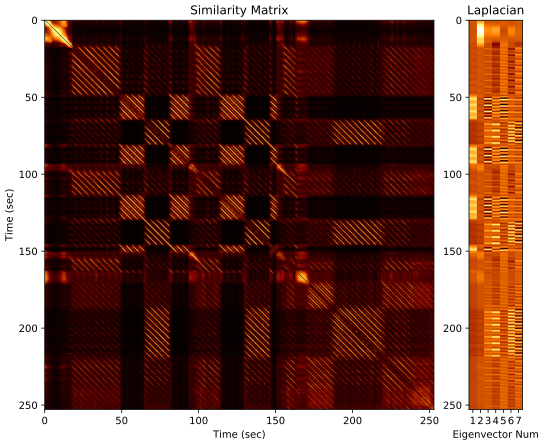
\includegraphics[width=\columnwidth]{SimilarityMatrix_Laplacian.pdf}
 \caption{Similarity matrix and Laplacian eigenvectors.}
 \label{fig:example}
\end{figure}


\begin{figure}
 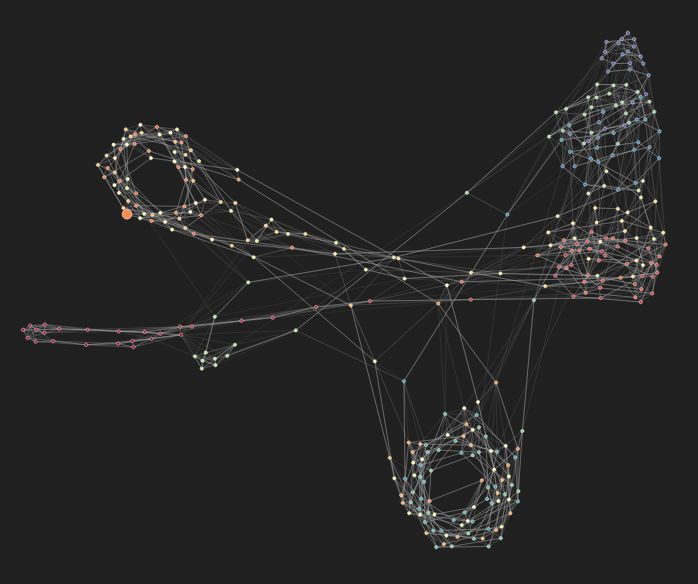
\includegraphics[width=\columnwidth]{ForceGraph.pdf}
 \caption{Force graph.}
 \label{fig:example}
\end{figure}

% For bibtex users:
\bibliography{main}


\end{document}
